\subsection{UML-Diagramm}
\label{subsec:uml}

\begin{figure}[hbtp]
\centering
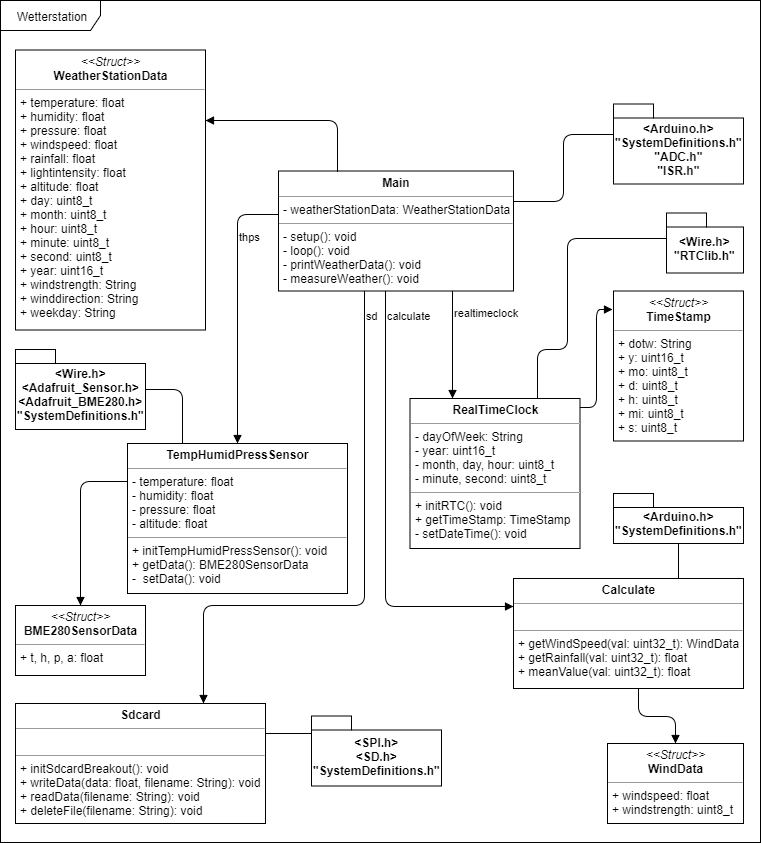
\includegraphics[width=\textwidth]{graphics/UML/UML_Diagramm_picture.PNG}
\caption{UML-Diagramm}
\label{fig:uml_diagramm}
\end{figure}

Das in der Abbildung \ref{fig:uml_diagramm} dargestellte UML-Diagramm soll den Aufbau und die logischen Zusammenhänge der Firmware visualisieren. Darin wird gezeigt, welche Headerfiles bei den Klassen benötigt werden. Zudem sind die Attribute, wie auch die Funktionen mit ihren Access Specifier, Argumenten und Rückgabewerten aufgelistet. \\

Durch diese Struktur ist es möglich, adaptiv mehrere Komponenten hinzuzufügen und anzupassen. Zudem könnten somit auch mehrere Sensoren vom gleichen Typ ohne grossen weiteren Aufwand implementiert werden.\\

\subsubsection{Lizenzen}
\label{subsubsec:lizenzen}

Die verwendeten Librarys sind grundsätzlich aus der Arduino IDE von Arduino. Arduino selbst ist eine aus Soft- und Hardware bestehende Physical-Computing-Plattform, bei welcher beide Komponenten auf Open-Source-Basis quelloffen sind \cite{arduinoWiki}. Nach Aussage von Arduino selbst, stehen alle C/C++ Mikrocontroller Librarys unter der \textbf{LGPL} \cite{ArduinoLicense2019}. Einige Lizenz-Texte stehen im Anhang \ref{sec:lizenztexte}. \\

%Die RTClib steht unter der \textbf{MIT}-Lizenz, zusätzlich befindet sich noch der Lizenz-Text im Anhang \ref{subsec:rtclib_lizenztext}. Auch der Lizenz-Text der Adafruit_BME280 ist im Anhang \ref{subsec:adafruit_bme280_lizenztext}.\\

\begin{table}[h]
\centering
\caption{Lizenzen}
\label{tab:lizenzen}
\begin{tabular}{|l|l|l|}
\hline 
\textbf{Library} & \textbf{Author} & \textbf{Lizenz} \\ 
\hline 
Arduino & Arduino Team & LGPL V2.1 \\ 
\hline 
SPI & Cristian Maglie, Paul Stoffregen, Matthijs Kooijman, Andrew J. Kroll & LGPL V2.1 \\ 
\hline 
Wire & Nicholas Zambetti, Todd Krein, Chuck Todd & LGPL V2.1 \\ 
\hline 
SoftwareSerial & Limor Fried, Mikal Hart, Paul Stoffregen, Garrett Mace, Brett Hagman & LGPL V2.1 \\ 
\hline 
SD & SparkFun Electronics & GPL V3 \\ 
\hline 
RTClib & JeeLabs & - \\ 
\hline 
Adafruit\_Sensor & Kevin Townsend & Apache V2.0 \\ 
\hline 
Adafruit\_BME280 & Kevin Townsend & BSD \\ 
\hline 
Adafruit\_FONA & Limor Fried & BSD \\ 
\hline 
Adafruit\_TSL2561\_U & Kevin Townsend & BSD \\ 
\hline 
\end{tabular} 
\end{table}
\todo[inline]{Schreiben: SD GPL wegen sdfatlib. Es hat da zwei drin, File.cpp und SD.cpp. JeeLabs angeben mit link http://news.jeelabs.org/code/. Die The Android Open Source Project hat bei Adafruit Sensor das Copyright. Vielleicht hinzuschreiben. Und zum schluss noch den Text überarbeiten.}